%%%%%%%%%%%%%%%%%%%%%%%%%%%%%%%%%%%%%%%%%
% Classicthesis Typographic Thesis
% LaTeX Template
% Version 1.1 (4/8/12)
%
% This template has been downloaded from:
% http://www.LaTeXTemplates.com
%
% Original author:
% André Miede (http://www.miede.de)
%
% License:
% CC BY-NC-SA 3.0 (http://creativecommons.org/licenses/by-nc-sa/3.0/)
%
% General Tips:
% 1) Make sure to edit the classicthesis-config.file
% 2) New enumeration (A., B., C., etc in small caps): \begin{aenumerate} \end{aenumerate}
% 3) For margin notes: \marginpar or \graffito{}
% 4) Do not use bold fonts in this style, it is designed around them
% 5) Use tables as in the examples
% 6) See classicthesis-preamble.sty for useful commands
%
%%%%%%%%%%%%%%%%%%%%%%%%%%%%%%%%%%%%%%%%%

%----------------------------------------------------------------------------------------
%	PACKAGES AND OTHER DOCUMENT CONFIGURATIONS
%----------------------------------------------------------------------------------------

\documentclass[
		twoside,openright,titlepage,numbers=noenddot,headinclude,%1headlines,
                footinclude=true,cleardoublepage=empty,
                BCOR=5mm,paper=a4,fontsize=11pt, % Binding correction, paper type and font size
                english, % Languages
                ]{scrreprt} 
                
% Includes the file which contains all the document configurations and packages - make sure to edit this file
%%%%%%%%%%%%%%%%%%%%%%%%%%%%%%%%%%%%%%%%%
% Thesis Configuration File
%
% The main lines to change in this file are in the DOCUMENT VARIABLES
% section, the rest of the file is for advanced configuration.
%
%%%%%%%%%%%%%%%%%%%%%%%%%%%%%%%%%%%%%%%%%

%----------------------------------------------------------------------------------------
%	DOCUMENT VARIABLES
%	Fill in the lines below to enter your information into the thesis template
%	Each of the commands can be cited anywhere in the thesis
%----------------------------------------------------------------------------------------

% Remove drafting to get rid of the '[ Date - classicthesis version 4.0 ]' text at the bottom of every page
\PassOptionsToPackage{eulerchapternumbers,listings,pdfspacing,subfig,beramono,eulermath,parts,dottedtoc,tocaligned}{classicthesis}
% Available options: drafting parts nochapters linedheaders eulerchapternumbers beramono eulermath pdfspacing minionprospacing tocaligned dottedtoc manychapters listings floatperchapter subfig
% Adding 'dottedtoc' will make page numbers in the table of contents flushed right with dots leading to them

\newcommand{\myTitle}{Tangible\xspace}
\newcommand{\mySubtitle}{A Python library to convert data into tangible 3D models.\xspace}
\newcommand{\myThesis}{Student Research Project Thesis\xspace}
\newcommand{\myName}{Danilo Bargen\xspace}
\newcommand{\myProf}{Prof. Dr. Josef M. Joller\xspace}
\newcommand{\myFaculty}{ITA Institute for Internet Technologies and Applications\xspace}
\newcommand{\myDepartment}{Department of Computer Science\xspace}
\newcommand{\myUni}{HSR University of Applied Science Rapperswil\xspace}
\newcommand{\myLocation}{Rapperswil\xspace}
\newcommand{\myTime}{Fall 2013\xspace}
\newcommand{\myVersion}{version 1.0\xspace}
\newcommand{\myLicense}{CC BY-SA 3.0 Unported\xspace}
\newcommand{\myKeywords}{3D Printing, CAD, Cross Compilers, Data Analysis, Data
Visualization, OpenSCAD, Python, Software Libraries, Statistics, Tangible}

%----------------------------------------------------------------------------------------
%	USEFUL COMMANDS
%----------------------------------------------------------------------------------------

\newcommand{\ie}{i.\,e.}
\newcommand{\Ie}{I.\,e.}
\newcommand{\eg}{e.\,g.}
\newcommand{\Eg}{E.\,g.} 

\newcommand{\tangible}{\emph{Tangible}}

\newcounter{dummy} % Necessary for correct hyperlinks (to index, bib, etc.)
\providecommand{\mLyX}{L\kern-.1667em\lower.25em\hbox{Y}\kern-.125emX\@}

%----------------------------------------------------------------------------------------
%	PACKAGES
%----------------------------------------------------------------------------------------

\usepackage{lipsum} % Used for inserting dummy 'Lorem ipsum' text into the template

%------------------------------------------------
 
\PassOptionsToPackage{utf8}{inputenc}
\usepackage{inputenc}
 
%------------------------------------------------

\PassOptionsToPackage{american}{babel}
\usepackage{babel}

%------------------------------------------------			

\PassOptionsToPackage{square,numbers}{natbib}
\usepackage{natbib}
 
%------------------------------------------------

\PassOptionsToPackage{fleqn}{amsmath} % Math environments and more by the AMS 
\usepackage{amsmath}
 
%------------------------------------------------

\PassOptionsToPackage{T1}{fontenc}
\usepackage{fontenc}

%------------------------------------------------

\usepackage{xspace} % To get the spacing after macros right

%------------------------------------------------

\usepackage{mparhack} % To get marginpar right

%------------------------------------------------

\usepackage{fixltx2e} % Fixes some LaTeX stuff 

%------------------------------------------------

\PassOptionsToPackage{smaller}{acronym} % Include printonlyused in the first bracket to only show acronyms used in the text
\usepackage{acronym} % nice macros for handling all acronyms in the thesis

%------------------------------------------------

%\renewcommand*{\acsfont}[1]{\textssc{#1}} % For MinionPro
\renewcommand{\bflabel}[1]{{#1}\hfill} % Fix the list of acronyms

%------------------------------------------------

\PassOptionsToPackage{pdftex}{graphicx}
\usepackage{graphicx} 
\usepackage{subfig}

%------------------------------------------------

\usepackage{pgf} 
\usepackage{tikz} 
\usepackage{tikz-qtree}
\usetikzlibrary{}

%------------------------------------------------

\usepackage{wrapfig}

%------------------------------------------------

\usepackage{siunitx}


%----------------------------------------------------------------------------------------
%	FLOATS: TABLES, FIGURES AND CAPTIONS SETUP
%----------------------------------------------------------------------------------------

\usepackage{tabularx} % Better tables
\setlength{\extrarowheight}{3pt} % Increase table row height
\newcommand{\tableheadline}[1]{\multicolumn{1}{c}{\spacedlowsmallcaps{#1}}}
\newcommand{\myfloatalign}{\centering} % To be used with each float for alignment
\usepackage{caption}
\captionsetup{format=hang,font=small}
\usepackage{subfig}  

%----------------------------------------------------------------------------------------
%	CODE LISTINGS SETUP
%----------------------------------------------------------------------------------------

\usepackage{minted} % Syntax highlighting                                                                                                                                                                                                      
\usemintedstyle{tango}
\definecolor{tango-bg}{HTML}{F8F8F8}

\newminted{python}{bgcolor=tango-bg,frame=lines,framesep=2mm,samepage=true,fontsize=\footnotesize}

%\usepackage{listings} 
%\lstset{emph={trueIndex,root},emphstyle=\color{BlueViolet}}%\underbar} % for special keywords
%\lstset{language=Python, % Specify the language for listings here
%keywordstyle=\color{RoyalBlue}, % Add \bfseries for bold
%basicstyle=\small\ttfamily, % Makes listings a smaller font size and a different font
%%identifierstyle=\color{NavyBlue}, % Color of text inside brackets
%commentstyle=\color{Green}\ttfamily, % Color of comments
%stringstyle=\rmfamily, % Font type to use for strings
%numbers=left, % Change left to none to remove line numbers
%numberstyle=\scriptsize, % Font size of the line numbers
%stepnumber=5, % Increment of line numbers
%numbersep=8pt, % Distance of line numbers from code listing
%showstringspaces=false, % Sets whether spaces in strings should appear underlined
%breaklines=true, % Force the code to stay in the confines of the listing box
%%frameround=ftff, % Uncomment for rounded frame
%frame=single, % Frame border - none/leftline/topline/bottomline/lines/single/shadowbox/L
%belowcaptionskip=.75\baselineskip % Space after the "Listing #: Desciption" text and the listing box
%}

%----------------------------------------------------------------------------------------
%	HYPERREFERENCES
%----------------------------------------------------------------------------------------

\PassOptionsToPackage{pdftex,hyperfootnotes=false,pdfpagelabels}{hyperref}
\usepackage{hyperref}  % backref linktocpage pagebackref
\pdfcompresslevel=9
\pdfadjustspacing=1

\hypersetup{
% Uncomment the line below to remove all links (to references, figures, tables, etc)
%draft, 
colorlinks=true, linktocpage=true, pdfstartpage=1, pdfstartview=FitV,
% Uncomment the line below if you want to have black links (e.g. for printing black and white)
%colorlinks=false, linktocpage=false, pdfborder={0 0 0}, pdfstartpage=1, pdfstartview=FitV, 
breaklinks=true, pdfpagemode=UseNone, pageanchor=true, pdfpagemode=UseOutlines,
plainpages=false, bookmarksnumbered, bookmarksopen=true, bookmarksopenlevel=1,
hypertexnames=true, pdfhighlight=/O, urlcolor=webbrown, linkcolor=RoyalBlue, citecolor=webgreen,
%------------------------------------------------
% PDF file meta-information
pdftitle={\myTitle},
pdfauthor={\textcopyright\ \myName, \myUni, \myFaculty},
pdfsubject={\mySubtitle},
pdfkeywords={\myKeywords},
pdfcreator={pdfLaTeX},
pdfproducer={LaTeX with hyperref and classicthesis}
%------------------------------------------------
}   

%----------------------------------------------------------------------------------------
%	BACKREFERENCES
%----------------------------------------------------------------------------------------

\usepackage{ifthen} % Allows the user of the \ifthenelse command
\newboolean{enable-backrefs} % Variable to enable backrefs in the bibliography
\setboolean{enable-backrefs}{false} % Variable value: true or false

\newcommand{\backrefnotcitedstring}{\relax} % (Not cited.)
\newcommand{\backrefcitedsinglestring}[1]{(Cited on page~#1.)}
\newcommand{\backrefcitedmultistring}[1]{(Cited on pages~#1.)}
\ifthenelse{\boolean{enable-backrefs}} % If backrefs were enabled
{
\PassOptionsToPackage{hyperpageref}{backref}
\usepackage{backref} % to be loaded after hyperref package 
\renewcommand{\backreftwosep}{ and~} % separate 2 pages
\renewcommand{\backreflastsep}{, and~} % separate last of longer list
\renewcommand*{\backref}[1]{}  % disable standard
\renewcommand*{\backrefalt}[4]{% detailed backref
\ifcase #1 
\backrefnotcitedstring
\or
\backrefcitedsinglestring{#2}
\else
\backrefcitedmultistring{#2}
\fi}
}{\relax} 

%----------------------------------------------------------------------------------------
%	AUTOREFERENCES SETUP
%	Redefines how references in text are prefaced for different 
%	languages (e.g. "Section 1.2" or "section 1.2")
%----------------------------------------------------------------------------------------

\makeatletter
\@ifpackageloaded{babel}
{
\addto\extrasamerican{
\renewcommand*{\figureautorefname}{Figure}
\renewcommand*{\tableautorefname}{Table}
\renewcommand*{\partautorefname}{Part}
\renewcommand*{\chapterautorefname}{Chapter}
\renewcommand*{\sectionautorefname}{Section}
\renewcommand*{\subsectionautorefname}{Section}
\renewcommand*{\subsubsectionautorefname}{Section}
}
\addto\extrasngerman{
\renewcommand*{\paragraphautorefname}{Absatz}
\renewcommand*{\subparagraphautorefname}{Unterabsatz}
\renewcommand*{\footnoteautorefname}{Fu\"snote}
\renewcommand*{\FancyVerbLineautorefname}{Zeile}
\renewcommand*{\theoremautorefname}{Theorem}
\renewcommand*{\appendixautorefname}{Anhang}
\renewcommand*{\equationautorefname}{Gleichung}
\renewcommand*{\itemautorefname}{Punkt}
}
\providecommand{\subfigureautorefname}{\figureautorefname} % Fix to getting autorefs for subfigures right
}{\relax}
\makeatother

%----------------------------------------------------------------------------------------

\usepackage{classicthesis} 

%----------------------------------------------------------------------------------------
%	CHANGING TEXT AREA 
%----------------------------------------------------------------------------------------

%\linespread{1.05} % a bit more for Palatino
%\areaset[current]{312pt}{761pt} % 686 (factor 2.2) + 33 head + 42 head \the\footskip
%\setlength{\marginparwidth}{7em}%
%\setlength{\marginparsep}{2em}%

%----------------------------------------------------------------------------------------
%	USING DIFFERENT FONTS
%----------------------------------------------------------------------------------------

%\usepackage[oldstylenums]{kpfonts} % oldstyle notextcomp
%\usepackage[osf]{libertine}
%\usepackage{hfoldsty} % Computer Modern with osf
%\usepackage[light,condensed,math]{iwona}
%\renewcommand{\sfdefault}{iwona}
%\usepackage{lmodern} % <-- no osf support :-(
%\usepackage[urw-garamond]{mathdesign} <-- no osf support :-(


\begin{document}

\frenchspacing % Reduces space after periods to make text more compact

\raggedbottom % Makes all pages the height of the text on that page

\selectlanguage{american} % Select your default language - e.g. american or ngerman

%\renewcommand*{\bibname}{new name} % Uncomment to change the name of the bibliography
%\setbibpreamble{} % Uncomment to include a preamble to the bibliography - some text before the reference list starts

\pagenumbering{roman} % Roman page numbering prior to the start of the thesis content (i, ii, iii, etc)

\pagestyle{plain} % Suppress headers for the pre-content pages

%----------------------------------------------------------------------------------------
%	PRE-CONTENT THESIS PAGES
%----------------------------------------------------------------------------------------

% Title Page

\begin{titlepage}
\begin{center}
\large

\hfill
\vfill

\begingroup
\color{OsmGreen}{\LARGE{\myTitle}}\\ \bigskip % Thesis title
\endgroup

{\myName} % Your name

\vfill


\mySubtitle \\ % Thesis subtitle
\myThesis, \myTime. \\

\vspace{2cm}


\includegraphics[width=5cm]{images/HSR_Logo_CMYK} \medskip


\end{center}
\end{addmargin}

\end{titlepage}
 % Main title page

% Back of the title page

\thispagestyle{empty}

\hfill

\vfill

\noindent\myName: \textit{\myTitle} 
\textcopyright\ \myTime

\bigskip

\noindent\spacedlowsmallcaps{Supervisors}: \\
\myProf
%\myOtherProf \\ 
%\mySupervisor

\medskip

\noindent\spacedlowsmallcaps{University}: \\
\myUni

\medskip

\noindent\spacedlowsmallcaps{Department}: \\
\myDepartment

\medskip

\noindent\spacedlowsmallcaps{Institute}: \\
\myFaculty

\medskip

\noindent\spacedlowsmallcaps{Location}: \\
\myLocation

\medskip

\noindent\spacedlowsmallcaps{Time Frame}: \\
\myTime

\medskip

\noindent\spacedlowsmallcaps{License}: \\
\myLicense
 % Back of the title page

%\cleardoublepage% Dedication

\thispagestyle{empty}
\refstepcounter{dummy}

\pdfbookmark[1]{Dedication}{Dedication} % Bookmark name visible in a PDF viewer

\vspace*{3cm}

\begin{center}
\emph{Ohana} means family. \\
Family means nobody gets left behind, or forgotten. \\ \medskip
--- Lilo \& Stitch    
\end{center}

\medskip

\begin{center}
Dedicated to the loving memory of Rudolf Miede. \\ \smallskip
1939\,--\,2005
\end{center} % Dedication page

%\cleardoublepage\include{front_back_matter/foreword} % Uncomment and create a Foreword.tex to include a foreword

\cleardoublepage% Abstract

\pdfbookmark[1]{Abstract}{Abstract} % Bookmark name visible in a PDF viewer

\begingroup
\let\clearpage\relax
\let\cleardoublepage\relax
\let\cleardoublepage\relax

\chapter*{Abstract} % Abstract name

In the past, making data tangible was a complicated, manual process. Digital 3D
representations of complex data have been around for quite a while, but they
were always confined to the digital world. Mostly because it was impractical to
convert a digital model to a physical representation.

With the advent of cheap, affordable 3D printers, this changed. It is now easy
to convert a purely digital model to a tangible, physical object. The missing
piece in the process of making data tangible is the conversion of data to a
digital 3D model.

This thesis wants to solve that problem by providing an easy to use software
library with ``batteries included'' that can convert arbitrary numeric data to
3D models. The library -- named \tangible{} -- is written in Python and provides
a set of predefined but customizable shapes, a few tools to preprocess data and
a backend implementation for OpenSCAD, an open source programmatic CAD software.

\tangible{} is implemented as a cross-compiler with a simple abstract syntax
tree (AST), a set of predefined shapes that build on top of the AST and an
interface that allows the creation of different code generation backends.

The library is ready to use, well tested and thoroughly documented. It has been
released under an open source license and is available online at
\url{https://github.com/dbrgn/tangible}.

\endgroup			

\paragraph{Keywords:}\mbox{}\\
\textit{\myKeywords}

\vfill
 % Abstract page

\cleardoublepage% Acknowledgements

\pdfbookmark[1]{Acknowledgements}{Acknowledgements} % Bookmark name visible in a PDF viewer

\bigskip

%-------------------------------------------------

\begingroup

\let\clearpage\relax
\let\cleardoublepage\relax
\let\cleardoublepage\relax

\chapter*{Acknowledgements} % Acknowledgements section text

We want to thank the following people for their support and contributions to the thesis.\\\\

\textbf{Prof Stefan Keller, IFS Institute for Software}, for his strong support with regular meetings, contacts in the OSM community and time and effort in checking this thesis.\\\\

\textbf{Dr Petr Pridal, Klokan Technologies GmbH}, for his strong support with intermediate technical decisions, project management, regular meetings, donating cloud infrastructure and the CDN infrastructure for hosting the final tiles.\\\\

\begin{figure}[H]
  \centering
  
\includegraphics[scale=0.3]{images/klokantech_logo.png}
  \caption*{\url{http://www.klokantech.com/}}
\end{figure}
\endgroup

 % Acknowledgements page

\pagestyle{scrheadings} % Show chapter titles as headings

\cleardoublepage% Table of Contents - List of Tables/Figures/Listings and Acronyms

\refstepcounter{dummy}

\pdfbookmark[1]{\contentsname}{tableofcontents} % Bookmark name visible in a PDF viewer

\setcounter{tocdepth}{2} % Depth of sections to include in the table of contents - currently up to subsections

\setcounter{secnumdepth}{3} % Depth of sections to number in the text itself - currently up to subsubsections

\manualmark
\markboth{\spacedlowsmallcaps{\contentsname}}{\spacedlowsmallcaps{\contentsname}}
\tableofcontents 
\automark[section]{chapter}
\renewcommand{\chaptermark}[1]{\markboth{\spacedlowsmallcaps{#1}}{\spacedlowsmallcaps{#1}}}
\renewcommand{\sectionmark}[1]{\markright{\thesection\enspace\spacedlowsmallcaps{#1}}}

\clearpage

\begingroup 
\let\clearpage\relax
\let\cleardoublepage\relax
\let\cleardoublepage\relax

%----------------------------------------------------------------------------------------
%	List of Figures
%----------------------------------------------------------------------------------------

\refstepcounter{dummy}

%\pdfbookmark[1]{\listfigurename}{lof} % Bookmark name visible in a PDF viewer

\listoffigures

\vspace*{8ex}
\newpage

%----------------------------------------------------------------------------------------
%	List of Tables
%----------------------------------------------------------------------------------------

\refstepcounter{dummy}
\listoftables

\vspace*{8ex}
\newpage
    
%-------------------------------------
%	List of Listings
%-------------------------------------

%\refstepcounter{dummy}

%\addcontentsline{toc}{chapter}{\lstlistlistingname} % Uncomment if you would like the list of listings to appear in the table of contents

%\pdfbookmark[1]{\lstlistlistingname}{lol} % Bookmark name visible in a PDF viewer
%
%\lstlistoflistings 
%
%\vspace*{8ex}
%\newpage
       
%----------------------------------------------------------------------------------------
%	Acronyms
%----------------------------------------------------------------------------------------
\refstepcounter{dummy}
\markboth{\spacedlowsmallcaps{Acronyms}}{\spacedlowsmallcaps{Acronyms}}
\chapter*{Acronyms}

\begin{acronym}[Acronyms]
\acro{OSM}{OpenStreetMap, free map}
\acro{ETL}{Extract, Transform and Load}
\acro{RUP}{Rational Unified Process}
\acro{GIS}{Geographic Information System}
\acro{GDAL}{Geospatial Data Abstraction Library}
\acro{WMS}{Web Map Service}
\acro{DRY}{Don't Repeat Yourself}
\acro{CI}{Continuous Integration}


\end{acronym}  

\newpage

%----------------------------------------------------------------------------------------
%	Glossary
%----------------------------------------------------------------------------------------
\refstepcounter{dummy}
\markboth{\spacedlowsmallcaps{Glossary}}{\spacedlowsmallcaps{Glossary}}
\chapter*{Glossary}

\begin{acronym}[Glossary]
\acro{Vector Tiles}{Packets of geographic data, packaged into pre-defined roughly-square shaped "tiles" for transfer over the web}
\acro{Data Style}{Description of feature classes such as landuse, water or roads}
\acro{Visual Style}{Definition of style rules for a specific schema, which is defined in the data style}
\acro{Feature Class}{Group of features with the same geometry type and attributes}
\acro{Layer}{Mapbox definition of a feature class}
\acro{Mapbox Streets}{Name of Mapbox's vector tile source}
\acro{MBTiles}{File format for storing map tiles in a single file}
\acro{GeoJSON}{File format for encoding a variety of geographic data structures}
\acro{Mapnik XML}{Stylesheet for the mapnik rendering engine}
\acro{CartoCSS}{Mapbox propritary cartographic styling language}
\acro{Mapbox GL}{Clientside rendering engine}
\acro{Web GL}{Javascript API for the graphics library in browsers}
\acro{Mapbox Studio Classic}{Client application to design custom maps}
\acro{OSM Bright}{Mapbox visual style}
\acro{Docker}{Operation system level virtualization on Linux}
\acro{Kitematic}{Client application for controlling docker containers}
\acro{Natural Earth}{Public map dataset}
\acro{OSM Planet}{All OpenStreetMap data in one file}






\end{acronym}  

\endgroup % Contents, list of figures/tables/listings and acronyms

\pagenumbering{arabic} % Arabic page numbering for thesis content (1, 2, 3, etc)
%\setcounter{page}{90} % Uncomment to manually start the page counter at an arbitrary value (for example if you wish to count the pre-content pages in the page count)

\cleardoublepage % Avoids problems with pdfbookmark

%--------------------------------
%	THESIS CONTENT - CHAPTERS
%--------------------------------

\part{Technical Report} % First part of the thesis
% Chapter 1

\chapter{Management Summary}

\label{ch:motivation} % For referencing the chapter elsewhere, use \autoref{ch:introduction} 

%----------------------------------------------------------------------------------------

This is necessary to show the added value of our project and help the understanding.

%----------------------------------------------------------------------------------------

\section{Goal}\label{sec:datavis}

Our project is focused on creating a free and Open Source vector tiles of Open Street Map that can easily used by developers, cartographers and designers to create their custom maps.
Through the use of Docker we can provide workflows that don’t need a complicate setup and are deployable across operating systems.


%----------------------------------------------------------------------------------------

\section{The Rise of Affordable 3D Printing}\label{sec:history-3dprinting}

Digital 3D representations of complex data have been around for quite a while
\cite{marcus:2003}, but they were always confined to the digital world.  Mostly
because it was impractical to convert a digital model to a physical
representation.

Industrial 3D printing and CNC milling have been available for about 3 decades,
but just until recently these machines were prohibitively expensive for regular
people that just wanted to visualize data. The only alternative was manual work.

\marginpar{The patent ``US5121329: Apparatus and method for creating
three-dimensional objects'' was granted to S. Scott Crump in 1992 and expired in
2009.}

During the last few years this changed. In 2009, US patent 5121329
\cite{us5121329:1992} expired, and with that prices for consumer-ready 3D
printers plummeted.

\begin{figure}[h]
	\centering
	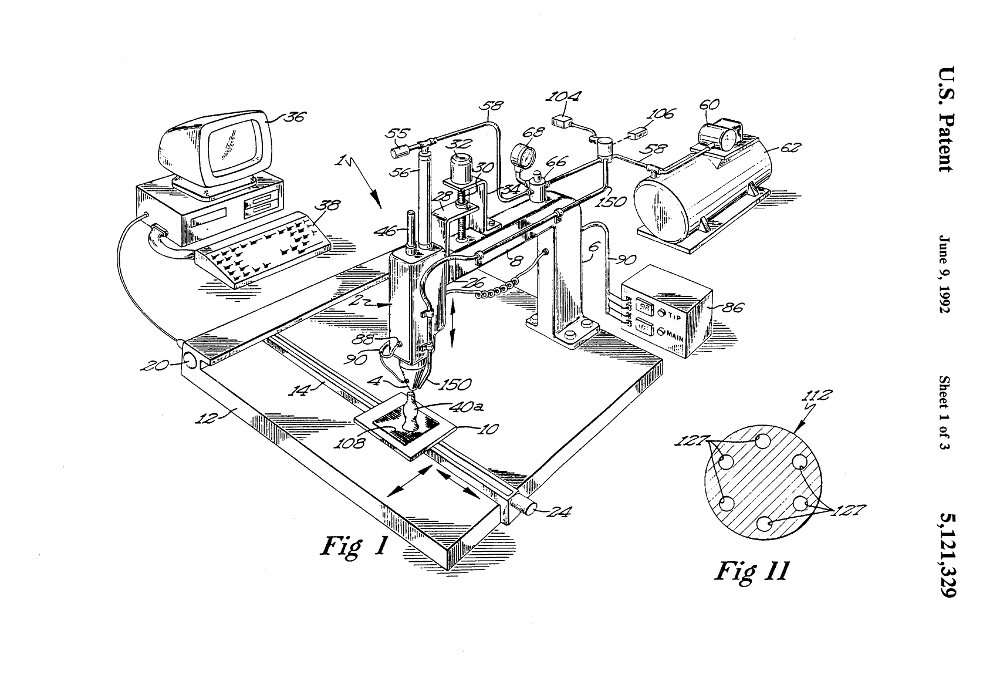
\includegraphics[width=\textwidth]{images/US5121329-1.png}
	\caption{US Patent 5121329}
	\label{img:us5121329a}
\end{figure}

\marginpar{The RepRap project works on creating general-purpose self-replicating
machines capable of printing plastic objects, and making them freely available
for the benefit of everyone.}

\noindent The surge of new cheap 3D printers -- as an affordable alternative to
the large, expensive industrial-grade machines -- was largely due to an
increasing number of enthusiasts from the \emph{Hacker-} and
\emph{Maker-}communities that worked on projects like the
RepRap\footnote{\url{http://reprap.org/wiki/RepRap}}, a very successful and
influential project.

As Erik De Bruijn, founder of the successful
Ultimaker\footnote{\url{https://www.ultimaker.com/}} company, discusses in his
Master's thesis \textit{``On the viability of the Open Source Development model
for the design of physical objects -- Lessons learned from the RepRap project''}
\cite{bruijn:2010}, the Open Source development model has proven to be well
suited in the field of physical fabrication.

At the same time, while many of these projects were started by communities as
non commercial Open Source\footnote{\url{http://opensource.org/}} and Open
Hardware\footnote{\url{http://www.oshwa.org/}} projects, crowdfunding platforms
like Kickstarter\footnote{\url{http://www.kickstarter.com/}} and
Indiegogo\footnote{\url{http://www.indiegogo.com/}} made raising capital for new
3D printers quick and easy, something that would not have been possible 10 years
ago. This resulted in a flood of readily assembled, affordable 3D printers even
for people lacking the skills to build their own machine from a list of parts.

%----------------------------------------------------------------------------------------

\section{From Data to Tangible Objects}

With the rapid and constantly accelerating developments in the field of 3D
printing, visualizing data as real, tangible objects has become feasible. There
are still some hurdles though.  The majority of people -- even those owning a 3D
printer -- have no experience with 3D modeling software. Most freely available
software tools to create 3D models -- like
OpenSCAD\footnote{\url{http://www.openscad.org/}} or
Blender\footnote{\url{http://www.blender.org/}} -- require a steep learning
curve and demand a nontrivial amount of learning time to create the desired
models. And platforms like
Thingiverse\footnote{\url{http://www.thingiverse.com/}} or
YouMagine\footnote{\url{https://www.youmagine.com/}} provide so many freely
available models that creating own objects is often not even a necessity.

Another aspect is that these general-purpose modeling tools are not optimized
for data visualization. Each type of visualization has to be created manually,
and when the data changes it's a lot of manual work to update the model.

\tangible{} was created to fill that void. It makes creation of customized,
printable data visualizations as 3D models easy, while at the same time
retaining a lot of flexibility for customization.


\cleardoublepage % Empty page before the start of the next part

%------------------------------------------------

\part{Project Documentation}

%------------------------------------------------

\part{Development Process}

%----------------------------------------------------------------------------------------
%	THESIS CONTENT - APPENDICES
%----------------------------------------------------------------------------------------

\appendix

\part{Appendix} % New part of the thesis for the appendix

%\include{chapters/0A} % Appendix A
%\include{chapters/0B} % Appendix B - empty template

%----------------------------------------------------------------------------------------
%	POST-CONTENT THESIS PAGES
%----------------------------------------------------------------------------------------

\cleardoublepage% Bibliography

\label{app:bibliography} % Reference the bibliography elsewhere with \autoref{app:bibliography}
\raggedright
\manualmark
\markboth{\spacedlowsmallcaps{\bibname}}{\spacedlowsmallcaps{\bibname}} 
\refstepcounter{dummy}

\addtocontents{toc}{\protect\vspace{\beforebibskip}} % Place the bibliography slightly below the rest of the document content in the table of contents
\addcontentsline{toc}{chapter}{\tocEntry{\bibname}}

\bibliographystyle{plainnat}
\bibliography{bibliography}
 % Bibliography

\cleardoublepage% Declaration

\refstepcounter{dummy}
\pdfbookmark[0]{Declaration}{declaration} % Bookmark name visible in a PDF viewer

\chapter*{Declaration} % Declaration section text

\thispagestyle{empty}

Hereby we acknowledge,

\begin{itemize}
		\item that we conducted this thesis by ourselves and without any external help,
			except with those, which are explicitly mentioned,
		\item that all used sources are cited academically correct, and 
		\item that I didn't use any copyright protected materials (e.g. images) in
			an unauthorized manner.
\end{itemize}

\bigskip
 
\noindent\textit{\myLocation, \myTime}

\bigskip

\begin{flushright}
    \begin{tabular}{m{8cm}}
    \hspace{1cm}
\includegraphics[width=.5\textwidth]{images/signature_lukas.jpg}
    \\ \hline
    \centering Lukas Martinelli, \today \\
    \end{tabular}
\end{flushright}

\begin{flushright}
    \begin{tabular}{m{8cm}}
    \hspace{2cm}
\includegraphics[width=.33\textwidth]{images/signature_manuel.png}
    \\ \hline
    \centering Manuel Roth, \today \\
    \end{tabular}
\end{flushright}


 % Declaration

%----------------------------------------------------------------------------------------

\end{document}
